\chapter{Abordagem de resolução do problema}
Todos os problemas possuem diferentes métodos de resolução. Em geral, existe sempre uma plétora de abordagens possíveis
para resolver um dado problema. Neste capítulo vamos
analisar em maior pormenor a abordagem e implementação
tomadas.
\section{Spacecheck.sh}
\textbf{spacecheck.sh} é o primeiro e mais complexo dos
scripts a desenvolver. Este tem por função o atravessar de
diversas diretorias e sub-diretorias, contabilizando o
espaço ocupado pelos ficheiros nelas contidos.
\subsection{Visão geral da implementação}
A implementação começa com uma procura de todas as
subdiretorias dos argumentos passados ao \verb|script|.
Depois, usando um \verb|while loop| é-nos possível iterar
por cada linha do resultado, ou seja, por cada subdiretoria
dos argumentos dados, e executar comandos sobre eles.

Ao realizar um \verb|find| em cada subdiretoria, podemos avaliar as
permissões de leitura através do seu exit code,
e a partir de aí perceber se o tamanho pode ser calculado na
sua totalidade, ou se há diretórios aos quais não temos
permissões de acesso, nas quais o espaço ocupado deve ser 
considerado "NA".
\begin{figure}[H]
    \centering
    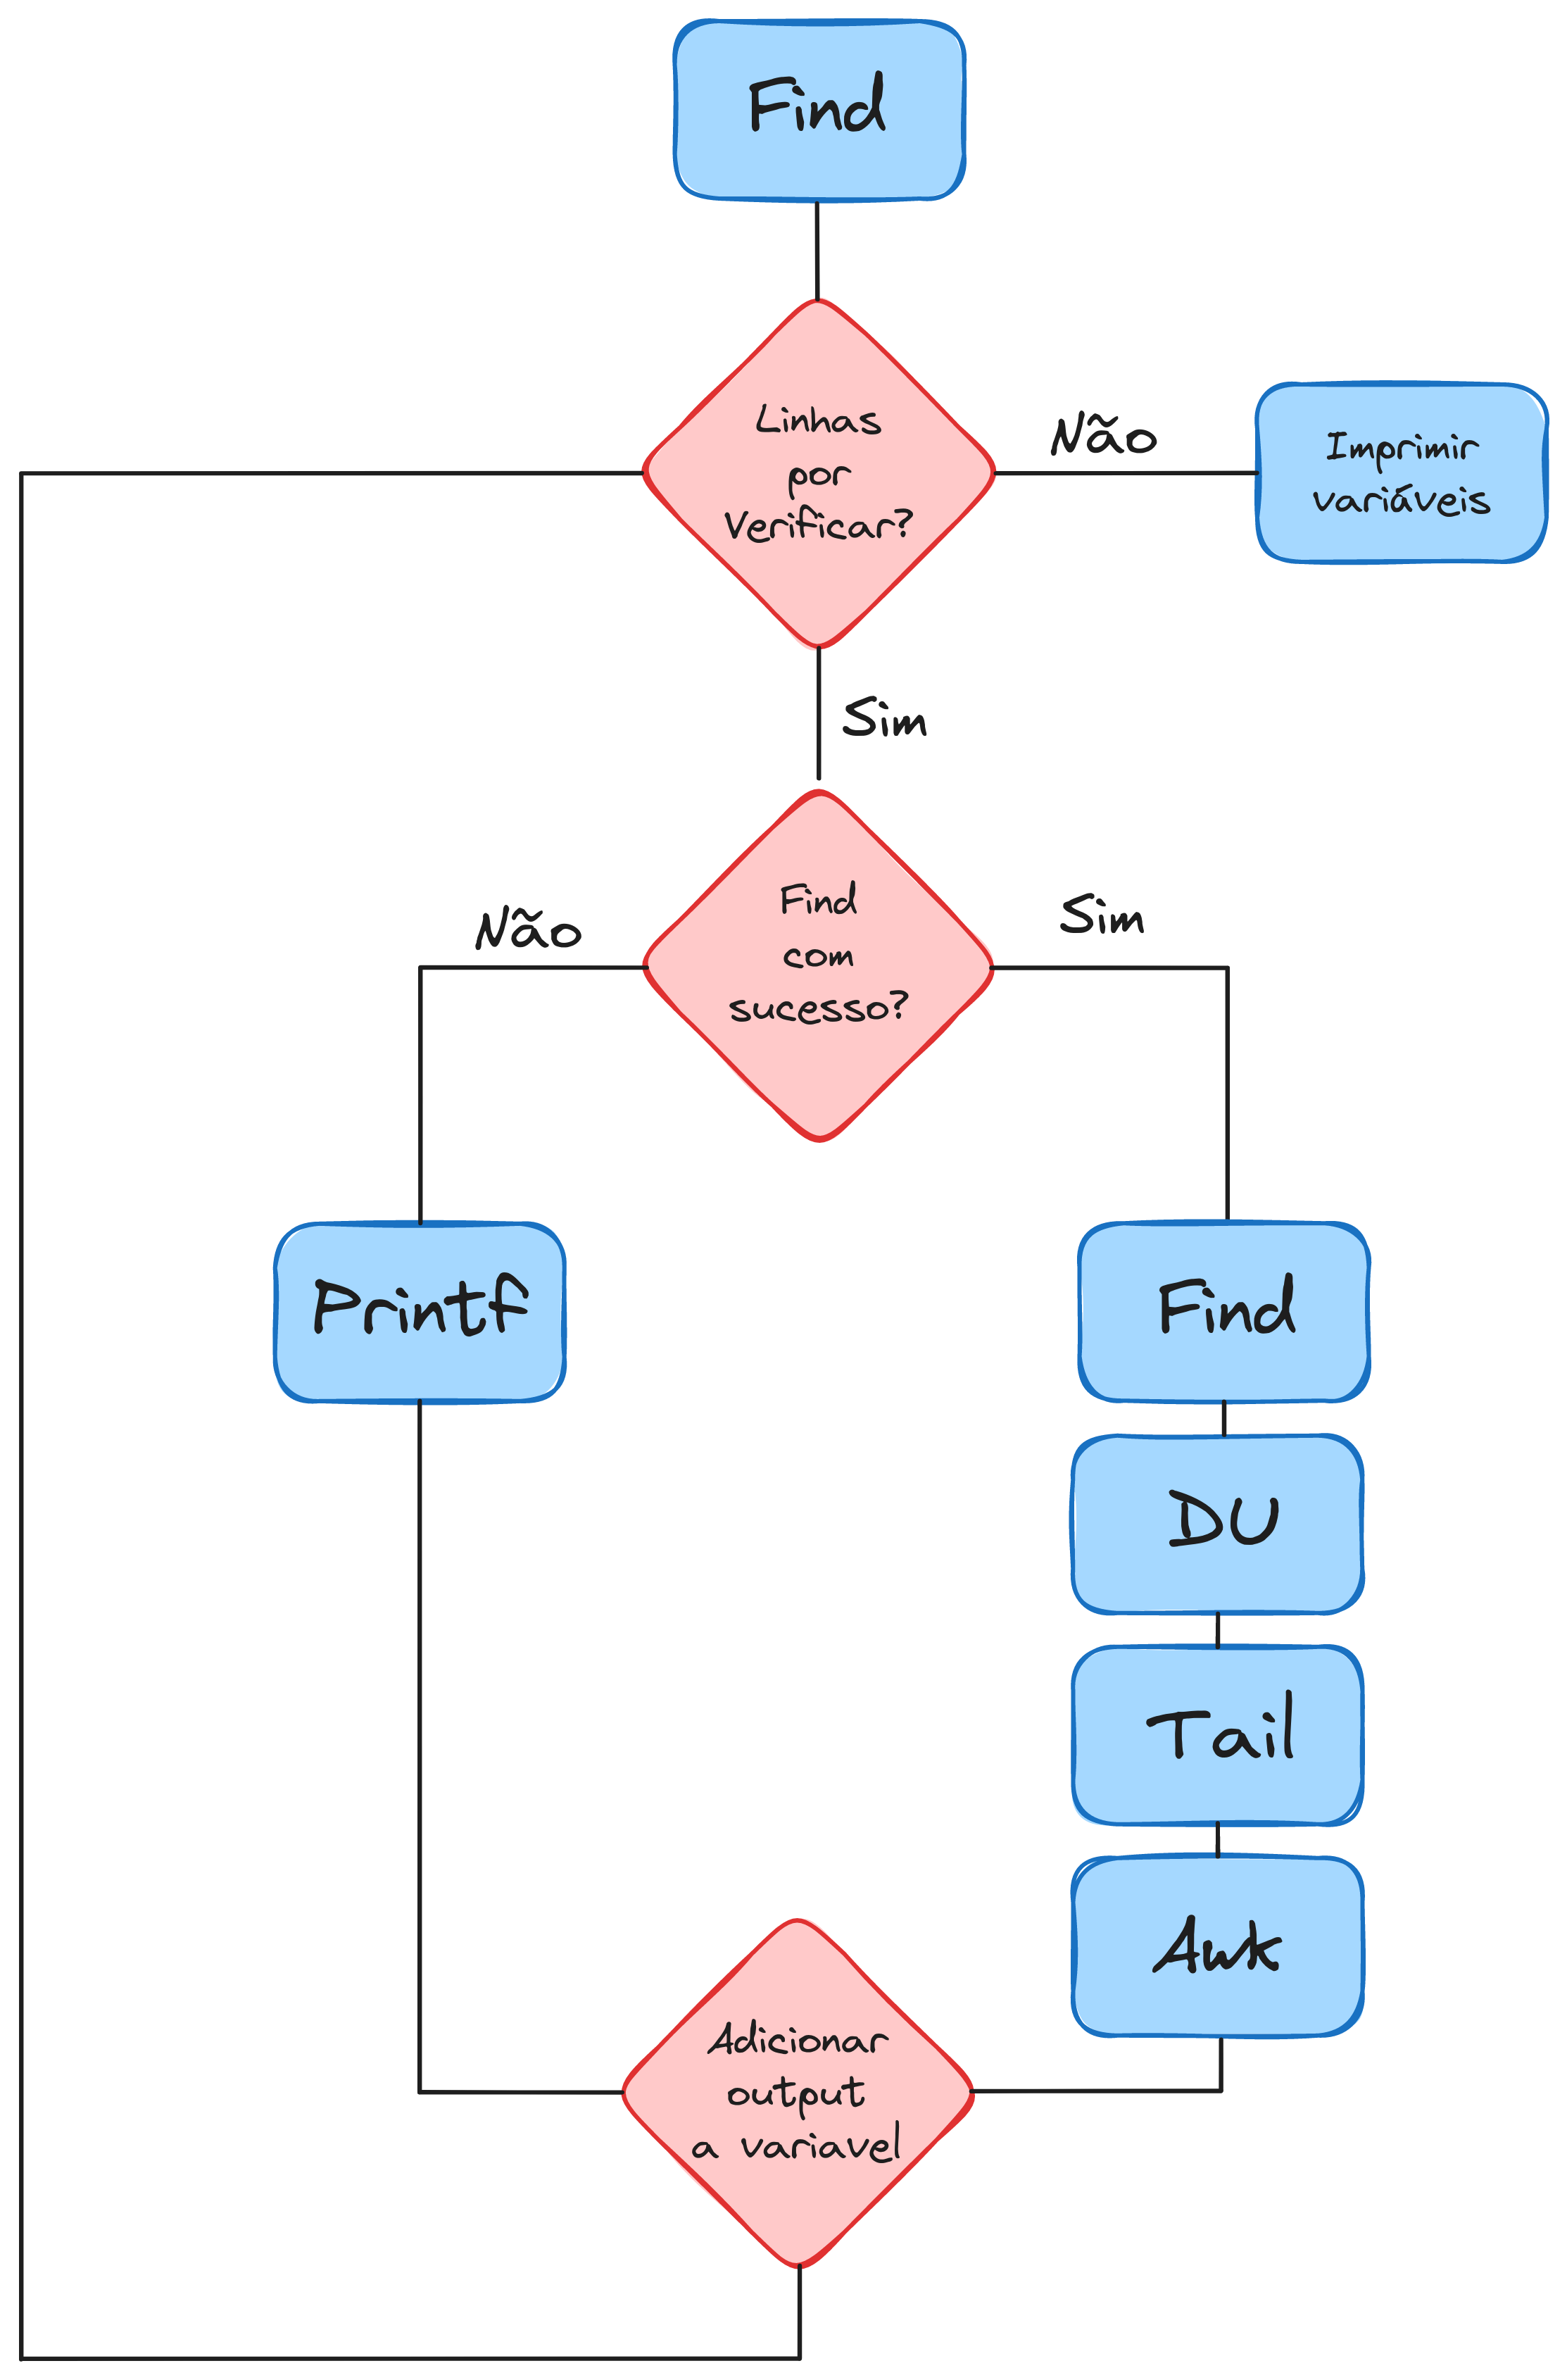
\includegraphics[height=13cm]{Fluxograma_Implementacao.png}
    \caption{Funcionamento do \textbf{spacecheck.sh}}
\end{figure}
Se o comando for bem-sucedido, podemos então executar uma
cadeia de comandos de modo a obter a totalidade do espaço
ocupado pela diretoria em estudo.
\subsection{Argumentos de Entrada}
   Ao efetuar a execução do \verb|script| é-nos possível
   introduzir alguns argumentos de entrada que nos permitem
   por um lado alterar o funcionamento do script e por outro
   alterar o modo como os resultados são apresentados ao
   utilizador.

   Os argumentos válidos (descritos em \ref{cap1.1} e
   \ref{cap1.3}) podem ser obtidos usando a utility
   \verb|getopts| num loop while (Código \ref{getopts}). Depois, podemos alterar
   certas variáveis para obter a funcionalidade desejada.

\begin{listing}[H]
\begin{minted}{bash}
while getopts ":harl:s:d:n:" o; do 
  case "$o" in
    a) sort_options="-k2 "
    ;;
    r) reverse_sort=1
    ;;
    s) find_size="+${OPTARG}c"
    ;;
    d) find_date="$(date --date "${OPTARG}" +%s)"
    ;;
    n) find_name+="${OPTARG}"
    ;;
    l) max_lines="${OPTARG}"
    ;;
  esac
done
shift $((OPTIND-1))
\end{minted}
\caption{Análise dos argumentos em \textbf{spacecheck.sh}}
\label{getopts}
\end{listing}

É, no entanto importante ter em conta a ordem do resultado,
pois por default se for ordenado por tamanho
será por ordem crescente, mas se for por nome será ordenado
por ordem alfabética, logo a opção (\textbf{-r}) terá
comportamentos diferentes baseado se é ordenado por nome ou
por tamanho.
Para tal, temos que avaliar se foi selecionada a opção de
ordenar por nome. Se tal aconteceu, então a variável \verb|reverse_sort| terá que se tornar no seu oposto lógico. Na
ausência de boleanos em bash, teremos que utilizar inteiros (Código \ref{invert-bool}) \cite{ebrahim2018mastering}. Caso estejamos a
ordenar por tamanho, então o comportamento padrão da flag é
ser verdadeira, e caso o utilizador introduza o argumento
\textbf{-r} então a flag passará a falsa.
\begin{listing}[H]
\begin{minted}{bash}
if [[ $sort_options != *"-k2"* ]]; then
  sort_options="-n -k1 "
  reverse_sort=$(( 1 - reverse_sort ))
fi

if [[ $reverse_sort == 0 ]]; then
  sort_options+="-r"
fi
\end{minted}
\caption{Inversão da variável reverse\_sort}
\label{invert-bool}
\end{listing}

\subsection{Verificação dos argumentos de entrada}

Alguns dos parâmetros de entrada carecem de verificação extra,
pois necessitam de um input do utilizador que nem sempre estará
correto. Então todos os parâmetros que necessitam deste input
terão que sofrer uma verificação dos seus argumentos.


Em todos os casos teremos que primeiro verificar se o valor
introduzido não é nulo, isto é, se foi de facto introduzido
algum valor (Código \ref{null-arg}):
\begin{listing}[H]
\begin{minted}{bash}
if [[ -z ${optarg} ]]; then
    echo "error: Option -* is missing an argument"
    print_help
    exit 1
fi
\end{minted}
\caption{Verificação da nulidade de um argumento}
\label{null-arg}
\end{listing}
De seguida, cada opção sofre uma verificação diferente,
dependendo da sua utilização. Por exemplo, na opção \verb|-d| a
data tem que ser válida (Código \ref{date-arg}), mas nas opções \verb|-l| e \verb|-s|
temos apenas que garantir que o valor é numérico e positivo (Código \ref{pos-num-arg}).
\begin{listing}[H]
\begin{minted}{bash}
if !(date -d "${OPTARG}") > /dev/null 2>&1; then
    echo "Error: Invalid date"
    print_help
    exit 1
fi
\end{minted}
\caption{Verificação de uma data}
\label{date-arg}
\end{listing}
\begin{listing}[H]
\begin{minted}{bash}
if ! [[ "${OPTARG}" == ?([[:digit:]]*) ]]; then
    echo "Error: Argument has to be a positive number"
    print_help
    exit 1
fi
\end{minted}
\caption{Verificação de um valor numérico positivo}
\label{pos-num-arg}
\end{listing}

Sobra por fim um caso específico, em que é escolhida a opção
\verb|-n|, mas não é introduzida uma expressão regular para
verificação de ficheiros. Em vez disso, a opção \verb|-n| é
seguida de um e apenas um diretório.
\begin{listing}[H]
    \centering
    \textbf{Exemplo:} \verb|./spacecheck.sh -n "./unit_tests"|
\end{listing}
Neste caso, o diretório seria consumido pela opção -n, e o
nosso script correria em todos os diretórios do computador. 
Então, para impedir tal caso, podemos só verificar se o número
de argumentos do programa após retirar as opções introduzidas é
nulo (Código \ref{verify-dirs}). Se tal acontecer, estamos perante o caso em questão,
tendo então que devolver um erro ao utilizador. 
Uma vantagem desta verificação é que impede também a chamada do
script sem qualquer argumento de entrada, ou diretório a analisar.
\begin{listing}[H]
    \centering
    \textbf{Exemplo:} \verb|./spacecheck.sh|
\end{listing}
\begin{listing}[H]
\begin{minted}{bash}
shift $((OPTIND-1))
if [[ "$#" == "0" ]]; then
    echo "An error has occured parsing the arguments"
    print_help
    exit 1
fi
\end{minted}
\caption{Verificação da existência de diretórios}
\label{verify-dirs}
\end{listing}

\subsection{Inicialização de variáveis}
A partir das seleções possíveis para ficheiros, seja por data
de modificação máxima, nome de ficheiro ou tamanho máximo,
podemos fazer três flags para cada uma, \verb|find_name|,
\verb|find_date| e \verb|find_size|, sendo que cada
variável, por padrão, assume valores que faz com que todos
os ficheiros sejam selecionados (Código \ref{init-vars}).

\begin{listing}[H]
\begin{minted}{bash}
find_name=".*"
find_size="+0"
find_date=$(date -d "n" +%s)
\end{minted}
\caption{Inicialiação de variáveis relacionadas com
argumentos}
\label{init-vars}
\end{listing}
\subsection{Seleção dos ficheiros a contabilizar}
Inicialmente é feito um \verb|find| para encontrar
diretorias e subdiretorias. O output é colocado num loop
\verb|while| de modo a ser-nos possível iterar por todas as
suas linhas, isto é, por todas as diretorias e
subdiretorias dos argumentos (Código \ref{get-dirs}).
\begin{listing}[H]
\begin{minted}{bash}

while IFS= read -r -d $'\0' folder; do 

done < <(find "$@" -type d -print0 2>/dev/null)
\end{minted}
\caption{Obtenção de diretorias e subdiretorias}
\label{get-dirs}
\end{listing}
De seguida, é necessário perceber se nós conseguimos ou não
aceder à diretoria em causa, pois se não tivermos permissões
de acesso não conseguimos calcular corretamente o tamanho
ocupado pela diretoria e os seus ficheiros no disco. Como
tal, podemos executar um comando \verb|find| na diretoria
e, dependendo do valor retornado, fazer a soma do espaço
ocupado pelos ficheiros ou apenas indicar o tamanho total
como sendo "NA" (Código \ref{perm-dir}).
\begin{listing}[H]
\begin{minted}{bash}
if find "$folder" >/dev/null 2>&1; then
    (...)
else
    error_output+="NA\t"$folder"\n"
fi
\end{minted}
\caption{Verificação da autorização de acesso à diretoria}
\label{perm-dir}
\end{listing}
Nos casos em que é possível aceder à diretoria, para
selecionar os ficheiros pedidos, as variáveis com as opções
de argumentos são passadas a um find presente no início da cadeia de comandos,
que procede a enviar todos os ficheiros selecionados para
du (Código \ref{select-files}).
\begin{listing}[H]
\begin{minted}{bash}
find "$folder" -type f -regex "^.*/$find_name$" \
! -newermt @"$find_date" -size "$find_size" -print0 \
\end{minted}
\caption{Seleção dos ficheiros a contabilizar}
\label{select-files}
\end{listing}
Note-se a maneira como o regex é passado ao find. Deste
modo, o find irá apenas contabilizar o nome do ficheiro para
comparação com o regex, pois ele irá dar match a todas as
\verb|/| até à ultima, onde encontra depois o nome do
ficheiro em estudo. Então, casos como a existência do padrão
de regex no path não serão considerados, sendo considerado
apenas o nome do ficheiro.
O du é depois configurado para aceitar por input o stdin
(usando o argumento \verb|-files0-from=-|), fazendo
automaticamente a contabilização e soma do espaço ocupado
por todos os ficheiros presentes no diretório (Código \ref{du}). O output é
depois processado com tail e awk para manter apenas os dados
desejados, e adicionado a uma variável que contém todo o
output dos casos em que é possível calcular o tamanho
ocupado pela diretoria.
\begin{listing}[H]
\begin{minted}{bash}
| du -c --files0-from=- -b --max-depth=0 | tail -n1 \ 
| awk '{print $1}'
\end{minted}
\caption{Contabilização do espaço ocupado}
\label{du}
\end{listing}
Para finalizar é só uma questão de imprimir os resultados,
tendo em conta as opções de sorteamento introduzidas pelo
utilizador
\begin{listing}[H]
\begin{minted}{bash}
printf "$regular_output" | sort $sort_options | head -n $max_lines
printf "$error_output" | sort $sort_options | head -n $max_lines
\end{minted}
\caption{Impressão dos resultados obtidos}
\end{listing}

\section{Spacerate.sh}
\textbf{spacerate.sh} é o segundo script a implementar. A
sua função é comparar dois outputs de \textbf{spacecheck.sh}
e retornar ao utilizador a variação de espaço ocupado por
cada diretoria em disco, destacando diretorias adicionadas
ou removidas entre a execução dos \verb|spacecheck's|
\subsection{Visão geral da implementação}
O \textbf{spacerate} é um script relativamente mais fácil de
implementar. O princípio básico desta implementação é 
a utilização de dois arrays associativos (Código
\ref{define-arrays}) \cite{ebrahim2018mastering}. Depois, podemos iterar cada array e
calcular a diferença entre o espaço ocupado em disco, tendo
em atenção a existência ou não das diretorias em ambos os
arrays associativos.
\begin{figure}[H]
    \centering
    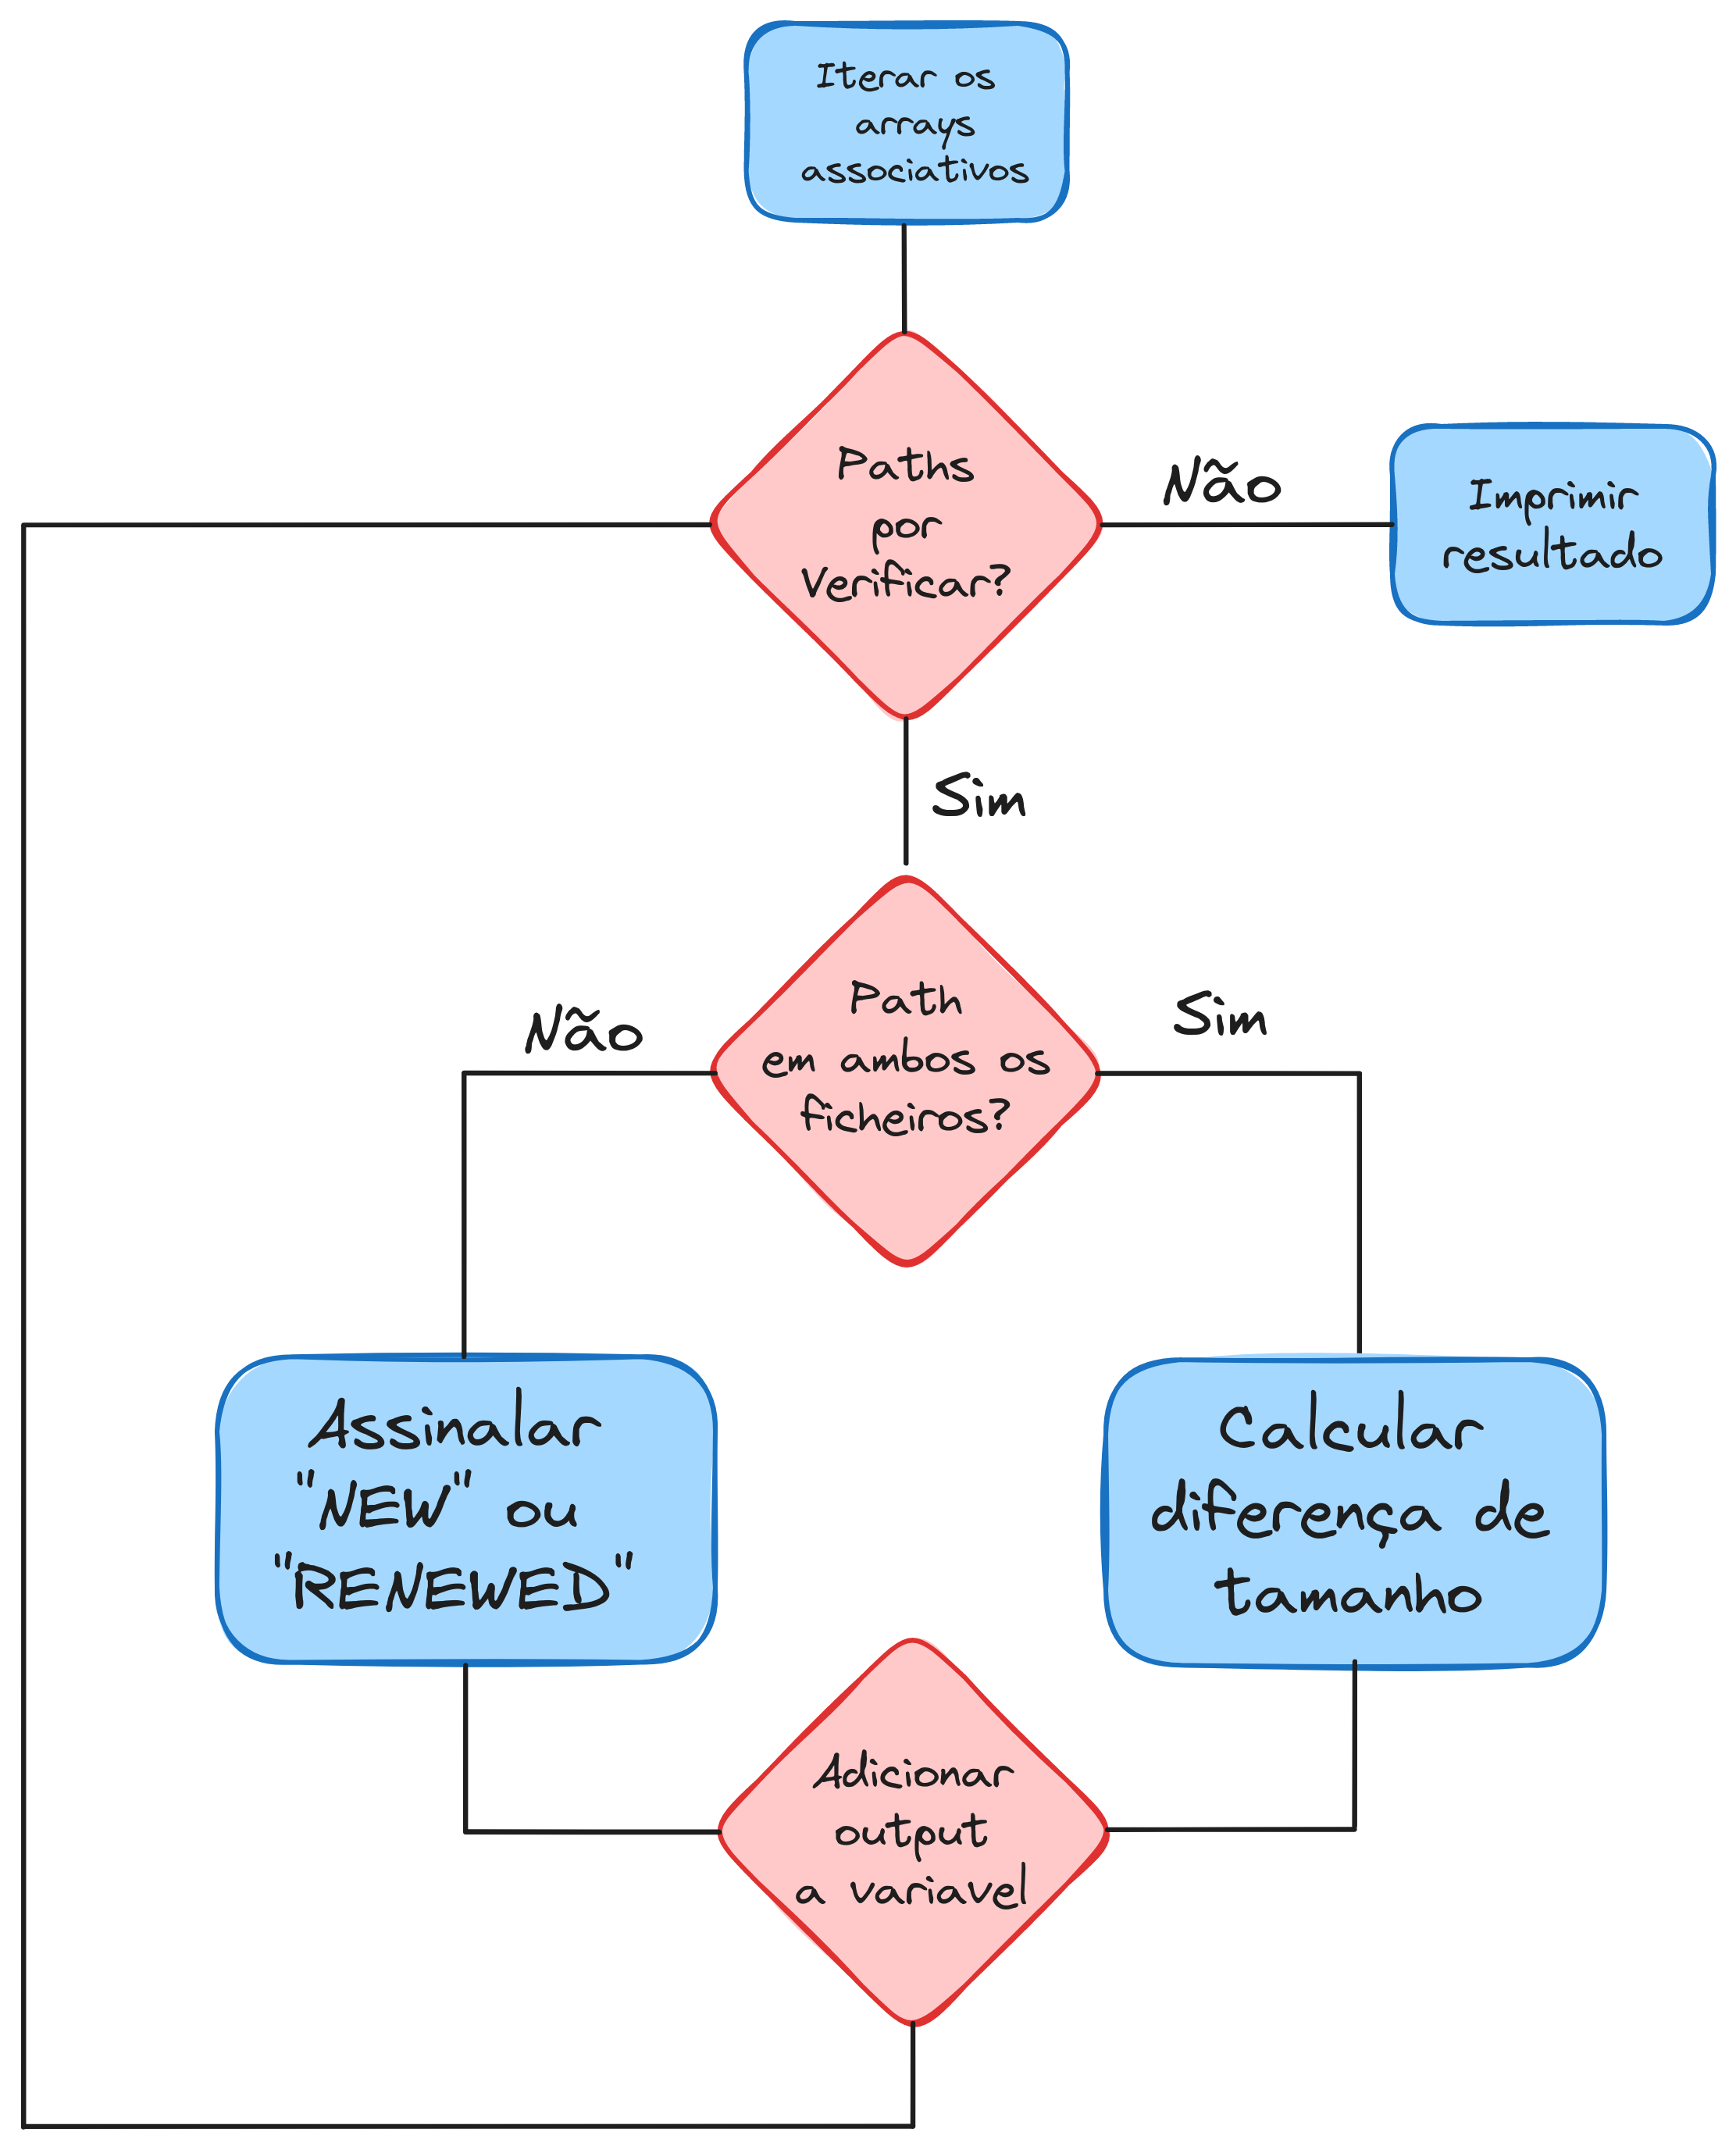
\includegraphics[height=13cm]{Fluxograma_Spacerate.png}
    \caption{Funcionamento do \textbf{spacecheck.sh}}
\end{figure}
\begin{listing}[H]
\begin{minted}{bash}
declare -A old_data
declare -A new_data
\end{minted}
\caption{Declaração dos arrays associativos}
\label{define-arrays}
\end{listing}
Cada array irá associar um path ao peso que tinha em cada ficheiro (Código \ref{add-files-arrays}).
Depois, podemos só comparar os valores armazenados em cada
array.
\begin{listing}[H]
\begin{minted}{bash}
$while IFS=$'\t' read -r size path; do
  old_data["$path"]=$size
done < <(tail -n +2 "$1") 

while IFS=$'\t' read -r size path; do
  new_data["$path"]=$size
done < <(tail -n +2 "$2");
\end{minted}
\caption{Adição das diretorias aos arrays associativos}
\label{add-files-arrays}
\end{listing}
\subsection{Comparação dos ficheiros}
Ao iterar o array \verb|old_data|, podemos obter o espaço
ocupado por cada diretório em cada um dos ficheiros, e
fazendo a diferença, obtemos o resultado expectado. Contudo,
temos que considerar o caso em que o path se encontra no
array \verb|old_data|, mas não no array \verb|new_data|. Caso
isto aconteça, é porque a totalidade do diretório foi
removido entre a criação dos ficheiros de registo. Como tal,
este pode ser assinalado como "REMOVED", e a diferença de
espaço será negativa e igual à totalidade do espaço ocupado pelo diretório (Código \ref{calc-occupied-space}).
\begin{listing}[H]
\begin{minted}{bash}
for key in "${!old_data[@]}"; do
  if [[ -v new_data["$key"] ]]; then
    new_value="${new_data["$key"]}"
    old_value="${old_data["$key"]}"
    if [[ "$new_value" != "NA" && "$old_value" != "NA" ]]; then
      difference=$((new_value - old_value))
    else
      difference="NA"
    fi
    output="$(printf "%s\t%s\n" "$difference" "$key")"
    result+="$output\n"
  else
    result+="$(printf "-${old_data["$key"]}\t$key\tREMOVED\n")\n"
  fi
done
\end{minted}
\caption{Cálculo da diferença de espaço ocupado}
\label{calc-occupied-space}
\end{listing}
Temos também que iterar pelas chaves do segundo array,
para obter todos os diretórios presentes no segundo
ficheiro, mas não no primeiro.
Caso isto aconteça, é porque o diretório foi criado entre a
criação dos ficheiros de registo, e como tal deve ser
assinalado como "NEW", sendo a diferença de espaço positiva
e igual à totalidade do espaço ocupado pela diretoria
atualmente (Código \ref{check-new-files}).
\begin{listing}[H]
\begin{minted}{bash}
for key in "${!new_data[@]}"; do
  if ! [[ -v old_data["$key"] ]]; then
    result+="$(printf "%s\t%s\tNEW\n" ${new_data["$key"]} "$key")\n"
  fi
done
\end{minted}
\caption{Verificação de ficheiros novos}
\label{check-new-files}
\end{listing}
Uma vez que todos os outputs foram guardados na variável
\verb|result|, podemos só imprimir essa variável para o
stdout, ordenada de acordo com as opções passadas por
argumentos ao script pelo utilizador (Código \ref{print-rate-result}).
\begin{listing}[H]
\begin{minted}{bash}
printf "$result" | sort $sort_options | head -n $max_lines
\end{minted}
\caption{Impressão do resultado obtido}
\label{print-rate-result}
\end{listing}
